
% 嘉应学院本科毕业论文Latex模板,来自: https://github.com/kkcocoon/JYUthesis/
% CTex下载地址 (要CTeX 3.0以上,windows选择x64.exe版的就行): https://ctex.org/ctex/download/ 

% 新手请注意:1.编译器一定要用XeLatex,涉及到中文的一般都要这个编译器
%            2.PDF与代码可交互

% 有参考文献的话,依次执行: 
% XeLatex       # 生成aux文件
% Biber         # 处理文献,右边的 B+ 快捷键
% XeLatex       # 插入文献引用
% XeLatex       # 最终编译

% 本文件的内容由嘉应学院 hkk 制作(2025年2月), zzk 修订(2025年8月)
% 有改进建议或代码疑问请邮件联系zzk0753@qq.com


\documentclass{JYU} % 模板样式文件在JYU.cls,修改更多细节需查询此文件
\Title{本科毕业论文\LaTeX 模板}{的使用方法} % 若标题一行,则第二个参数的文字删掉(注意花括号保留)
\author{张三} % 名字
\major{数学与应用数学} % 专业
\studentID{123456789} % 学号
\teacher{李四} % 指导老师
\GraduationYear{2026} % 2026届

\begin{document}
    \makecover
    % 承诺书中的学生签名图片位置,导师签名图片位置,签名日期(填答辩前的)
    \commitment{./图片/签名/空白签名.png}{./图片/签名/空白签名.png}{2025年5月1日}
    \cleardoublepage 
    \pagenumbering{Roman}
    \section*{摘要}
    \addcontentsline{toc}{section}{摘要} % 摘要添加到目录
    % 摘要:注意摘要是讲怎么做这个问题,得到了什么结果。不要写太多为什么做这个问题
	本科毕业论文是本科生培养体系中的关键一环,是毕业前夕全面检验学生综合实践能力与专业素养的必要步骤。但实际情况是,不少同学撰写的毕业论文质量欠佳,尤其在论文格式方面问题较为突出。本文聚焦于本科毕业论文 \LaTeX {} 模板的使用方法展开探讨。详细阐述了在运用该模板时,数学公式、表格、图片的格式规范,介绍了数学环境的正确搭建方式,同时也说明了参考文献格式的书写要求。旨在为同学们提供清晰、实用的指引,助力大家规范、高效地完成毕业论文写作,提升论文整体质量。
    
    \vspace{0.2cm}	
    \noindent{\bf 关键词: }{\hspace{0.08cm}毕业论文;~论文排版;~参考文献}
	
    \clearpage
    \section*{Abstract}
    \addcontentsline{toc}{section}{Abstract} % 添加到目录
	% 英文摘要:建议最好快完稿的时候写英文摘要
	The undergraduate thesis project is a crucial part of the undergraduate training program and a necessary step to comprehensively assess students' comprehensive practical abilities and professional qualities before graduation. However, the theses written by many students are of relatively poor quality, especially in terms of thesis formatting. 
	This paper explores the usage methods of the LaTeX template for undergraduate theses. It details the writing rules for mathematical formulas, table formats, picture formats, mathematical environments, and reference formats. The aim is to provide clear and practical guidance to help students complete their thesis writing in a standardized and efficient manner, thereby enhancing the overall quality of their theses. 
    
    \vspace{0.2cm}	
    \noindent{\textbf{Keywords:}\hspace{0.16cm}}Undergraduate Thesis;~Paper Typesetting;~References

	\cleardoublepage % 目录页单页开始
	\tableofcontents % 加入目录页
	
	\cleardoublepage % 单页开始
	\setcounter{page}{1} % 页码开始为1
	\pagenumbering{arabic} % 页码开始为罗马数字
    
\section{引言}

大学生毕业论文的撰写至关重要,主要体现在两个关键层面。其一,它是对学生知识储备与能力的一次全方位考察,能够全面反映学生在大学期间的学习成果。其二,这也是对学生进行科学研究基础训练的重要途径,有助于提升学生综合运用专业知识的能力,为毕业后求职就业奠定坚实基础,更为未来撰写专业学术论文积累宝贵经验。

在毕业论文的写作过程中,合理运用排版工具是确保论文质量的核心要素。目前,写作过程中普遍存在以下常见问题:
\begin{enumerate}[label=(\arabic*)]
	\item 数学公式排版杂乱无章,编号引用缺乏规范性,影响论文的专业性与严谨性;
	\item 图片与表格的格式不够美观,且常常缺少必要的说明信息,降低了论文的可读性;
	\item 参考文献的管理效率低下,导致文献引用的准确性和完整性难以保证;
	\item 代码附录的格式不统一,给读者的阅读和理解带来了不便。
\end{enumerate}

学术论文的排版是 \LaTeX{} 的核心竞争力之一,相关领域已取得了一系列重要研究成果。早期研究就已明确指出,相较于传统文字处理软件,\LaTeX{} 在数学符号排版方面优势显著\cite{KJYU201010018}。随着技术的不断进步,闫等人\cite{BJXB201303037}通过对比实验证实,\LaTeX{} 处理复杂公式的效率比主流办公软件显著提高。近年来,罗等人\cite{JYKQ201611011}开发的中文模板实现了数学符号与汉字的完美融合;刘等人\cite{DNZS201933114}进一步提出了公式排版的五项黄金准则;最新研究\cite{JYRJ202212005}更是开发出智能排版系统,实现了专业级别的公式排版。

本文聚焦于毕业论文中 \LaTeX{} 模板的使用方法展开深入研究,并提出了一系列适用于本科毕业论文排版的格式规范。 

\section{\LaTeX{}模板的使用方法}

\subsection{数学公式规范}

\subsubsection{第三级标题}

\textbf{(一)第四级标题}

\textbf{(1)第五级标题}

\textbf{1)第六级标题}

行内公式示例:损失函数定义为$L = \frac{1}{N}\sum_{i=1}^N(y_i-\hat{y}_i)^2$。

带编号公式:
\begin{equation}
	\frac{\partial L}{\partial w} = \frac{2}{N}\sum_{i=1}^N x_i(\hat{y}_i - y_i)
	\label{eq_loss_diff}
\end{equation}
公式\eqref{eq_loss_diff}是损失函数的导数。

不带编号的单独一行居中的公式:
\begin{equation*}
	1 + (\frac{1}{1-x^2})^3 
\end{equation*}

使用align环境实现多行公式对齐:
\begin{align}
	f(x) &= \int_{-\infty}^\infty \hat{f}(\xi)e^{2\pi i \xi x} \,d\xi \notag \\ 
	&= \sum_{n=0}^\infty \frac{(ix)^n}{n!}\int_{-\infty}^\infty \xi^n\hat{f}(\xi)\,d\xi 
	\label{eq_fourier}
\end{align}

\begin{equation*}
	\begin{split}
		&\min_{c_{m,j}^{L},c_{i,j}^{V}} \,\, \tau_{av} \\
		&s.t.\quad  
		\left\{\begin{array}{lc}
			\sum_{j=1}^{J}c_{i,j}^{V}\leq S^V    \\
			\sum_{j=1}^{J}c_{m,j}^{L}\leq S^L    \\
			c_{i,j}^{V}\in \left \{0,1\right \}  \\
			c_{m,j}^{L}\in \left \{0,1\right \}  \\
		\end{array}\right.
	\end{split}
\end{equation*}

cases环境处理分段函数:
\[
\text{ReLU}(x) = 
\begin{cases}
	0 & \text{当 } x < 0 \\
	x & \text{当 } x \geq 0
\end{cases}
\]

矩阵示例:
\[
\mathbf{J} = 
\begin{pmatrix}
	\frac{\partial f_1}{\partial x_1} & \cdots & \frac{\partial f_1}{\partial x_n} \\
	\vdots & \ddots & \vdots \\
	\frac{\partial f_m}{\partial x_1} & \cdots & \frac{\partial f_m}{\partial x_n}
\end{pmatrix}
\]

附录\ref{append_python}是相应的Python求解代码。


\subsection{表格图片使用规范}
表\ref{tab_algo}展示了优化算法的比较。注意每个表格要在正文中引用和详细说明, 不能出现没有标题或引用的表格,不要说“如下表1:”。
\begin{table}[!htbp]
	\caption{优化算法比较}
	\label{tab_algo}
	\centering
	\begin{tabular}{lccc}
		\toprule[1.5pt]
		\textbf{算法} & \textbf{准确率} & \textbf{训练时间(s)} & \textbf{内存占用(MB)} \\
		\midrule[1pt]
		SGD & 92.3\% & 120 & 850 \\
		Adam & 95.6\% & 150 & 920 \\
		RMSProp & 94.8\% & 140 & 890 \\
		\bottomrule[1.5pt]
	\end{tabular}
\end{table}

表\ref{tab_class}展示了跨列表格的使用方法。
\begin{table}[!htbp]
	\caption{多列合并示例}
	\label{tab_class}
	\centering
	\begin{tabular}{cccc}
		\toprule
		\multirow{2}{*}{\textbf{模型}} & \multicolumn{3}{c}{\textbf{评估指标}} \\
		\cmidrule{2-4}
		& 精确率 & 召回率 & F1值 \\
		\midrule
		SVM & 0.85 & 0.82 & 0.83 \\
		CNN & 0.92 & 0.91 & 0.91 \\
		\bottomrule
	\end{tabular}
\end{table}


\begin{figure}[!htbp]
	\centering
	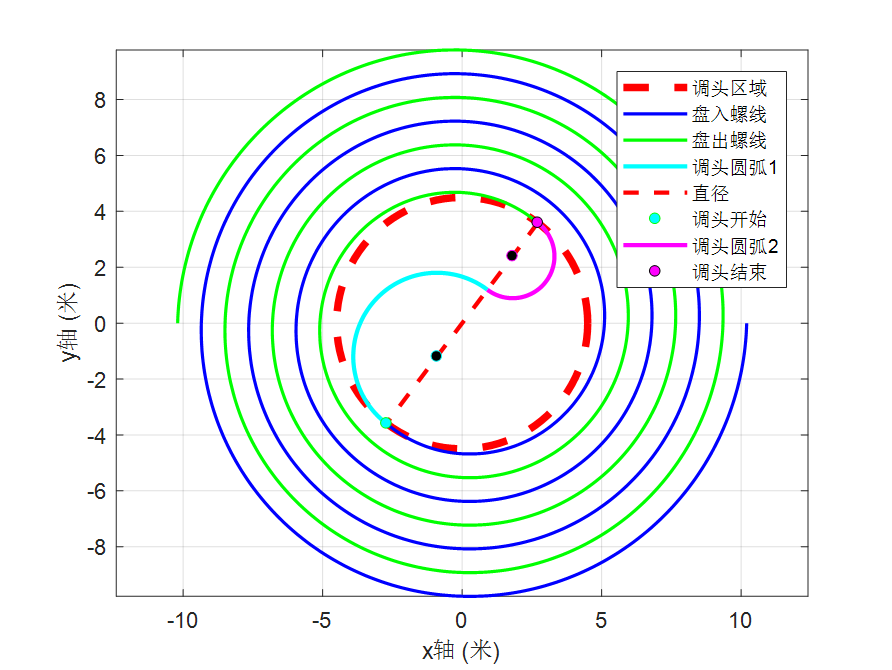
\includegraphics[width=0.8\textwidth]{./图片/论文图片/fig_track.png}
	\caption{螺线的盘入、调头和盘出的运动轨迹}\label{fig_track}
\end{figure}

图\ref{fig_track}展示了舞龙队的运动轨迹,分为四段:
\begin{itemize}
	\item 盘入螺线(蓝色):龙头从外围沿等距螺线向内旋转,逐渐靠近调头区域;
	\item 第一个圆弧(浅蓝色):龙头进入调头区域后,沿着半径为3米的圆弧开始调头;
	\item 第二个圆弧(紫色):龙头继续调头,沿着半径为1.5米的圆弧完成调头路径;
	\item 盘出螺线(绿色):调头完成后,龙头沿着与盘入螺线对称的螺旋线向外移动。
\end{itemize}
图中的红色区域为调头范围,并标出了各关键位置(起点、终点等),确保轨迹在调头时平滑衔接。

注意每个图片要在正文中引用和详细说明, 不能出现没有标题或引用的图片。 不要说“如下图1:” ,要用“如图1。”。

图\ref{fig_eval}是分类模型评估图,展示了如何使用子图排版。
\begin{figure}[!htbp]
	\centering
	\begin{subfigure}[b]{0.45\textwidth}
		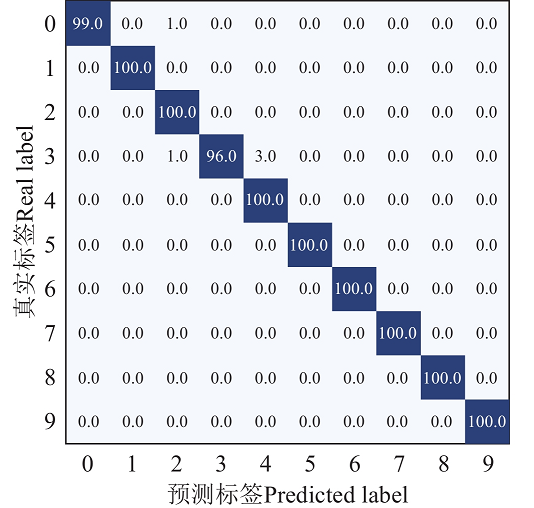
\includegraphics[width=\textwidth]{./图片/论文图片/fig_confusion.png}
		\caption{混淆矩阵}
	\end{subfigure}
	\begin{subfigure}[b]{0.45\textwidth}
		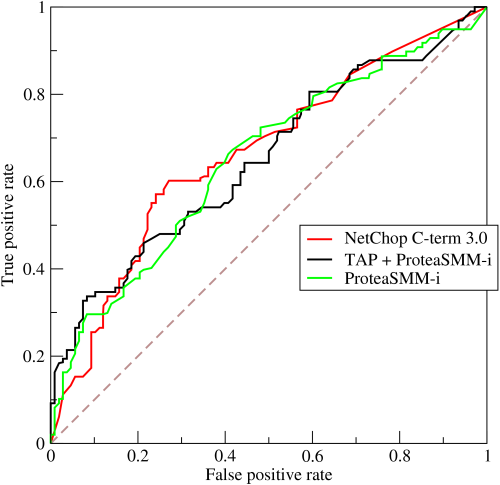
\includegraphics[width=\textwidth]{./图片/论文图片/fig_roc.png}
		\caption{ROC曲线}
	\end{subfigure}
	\caption{分类模型评估}
	\label{fig_eval}
\end{figure}

\subsection{数学环境使用规范}
本模板预定义了多种数学环境,适用于不同理论场景的规范排版。

\begin{definition}[欧几里得空间]\label{def:euclid}
	欧几里得空间是带有正定对称双线性形式的有限维实向量空间。
\end{definition}

\begin{theorem}[勾股定理]\label{thm:pythagoras}
	在直角三角形中,斜边的平方等于两直角边的平方和:
	\begin{equation}
		c^2 = a^2 + b^2
	\end{equation}
\end{theorem}

\begin{lemma}[Zorn引理]\label{lem:zorn}
	设$(P,\leq)$是非空偏序集,若$P$中每个链都有上界,则$P$至少有一个极大元。
\end{lemma}

\begin{corollary}[三角不等式]\label{col:triangle}
	对于任意实数$x,y$,成立:
	\begin{equation}
		|x+y| \leq |x| + |y|
	\end{equation}
\end{corollary}

\begin{assumption}[光滑性假设]\label{ass:smooth}
	本文假设所有函数在定义域内连续可微。
\end{assumption}

\begin{conjecture}[孪生素数猜想]\label{conj:twinprime}
	存在无穷多个素数$p$,使得$p+2$也是素数。
\end{conjecture}

\begin{axiom}[选择公理]\label{axi:choice}
	对任何由非空集合组成的集合族,都存在选择函数。
\end{axiom}

\begin{principle}[最小作用量原理]\label{pri:action}
	真实运动使作用量泛函取得极值。
\end{principle}

\begin{problem}[旅行商问题]\label{pro:tsp}
	给定城市集合及两两距离,求访问每座城市一次并返回起点的最短回路。
\end{problem}

\begin{example}[黎曼积分]\label{ex:riemann}
	函数$f(x)=x^2$在区间$[0,1]$的黎曼积分:
	\begin{equation}
		\int_0^1 x^2 dx = \frac{1}{3}
	\end{equation}
\end{example}

\begin{solution}[特征方程法]\label{sol:characteristic}
	求解微分方程$y''+py'+qy=0$的步骤:
	\begin{enumerate}
		\item 写出特征方程$\lambda^2+p\lambda+q=0$
		\item 根据根的情况确定通解形式
	\end{enumerate}
\end{solution}

\begin{proof}[勾股定理证明]
	如定义\ref{def:euclid}所述,在欧氏空间构造边长为$a,b,c$的直角三角形...(详细证明过程)
\end{proof}


建议使用 “algorithm” 环境排版算法,适用于伪代码、流程图等内容的规范展示。

\begin{algorithm}[!htbp]
	\caption{梯度下降算法}\label{alg:gradient_descent}
	\begin{algorithmic}[1]
		\REQUIRE 数据集 $X \in \mathbb{R}^{m \times n}$, 标签 $y \in \mathbb{R}^m$, 学习率 $\eta$, 最大迭代次数 $T$
		\ENSURE 模型参数 $w \in \mathbb{R}^n$
		\STATE 初始化参数 $w \gets \mathbf{0}$
		\FOR{$t = 1$ \TO $T$}
		\STATE 计算梯度:$\nabla_w L \gets \frac{2}{m} X^\top (Xw - y)$
		\STATE 更新参数:$w \gets w - \eta \nabla_w L$
		\IF{$\|\nabla_w L\| < \epsilon$}
		\STATE \textbf{break} \COMMENT{收敛条件}
		\ENDIF
		\ENDFOR
		\RETURN $w$
	\end{algorithmic}
\end{algorithm}


算法\ref{alg:gradient_descent}展示了梯度下降算法的伪代码实现,其中:
\begin{itemize}
	\item 第1-2行定义了输入和输出;
	\item 第3行初始化模型参数;
	\item 第4-8行通过迭代更新参数;
	\item 第9行返回最终结果。
\end{itemize}

\subsection{参考文献使用规范}
\begin{figure}[!htbp]
	\centering
	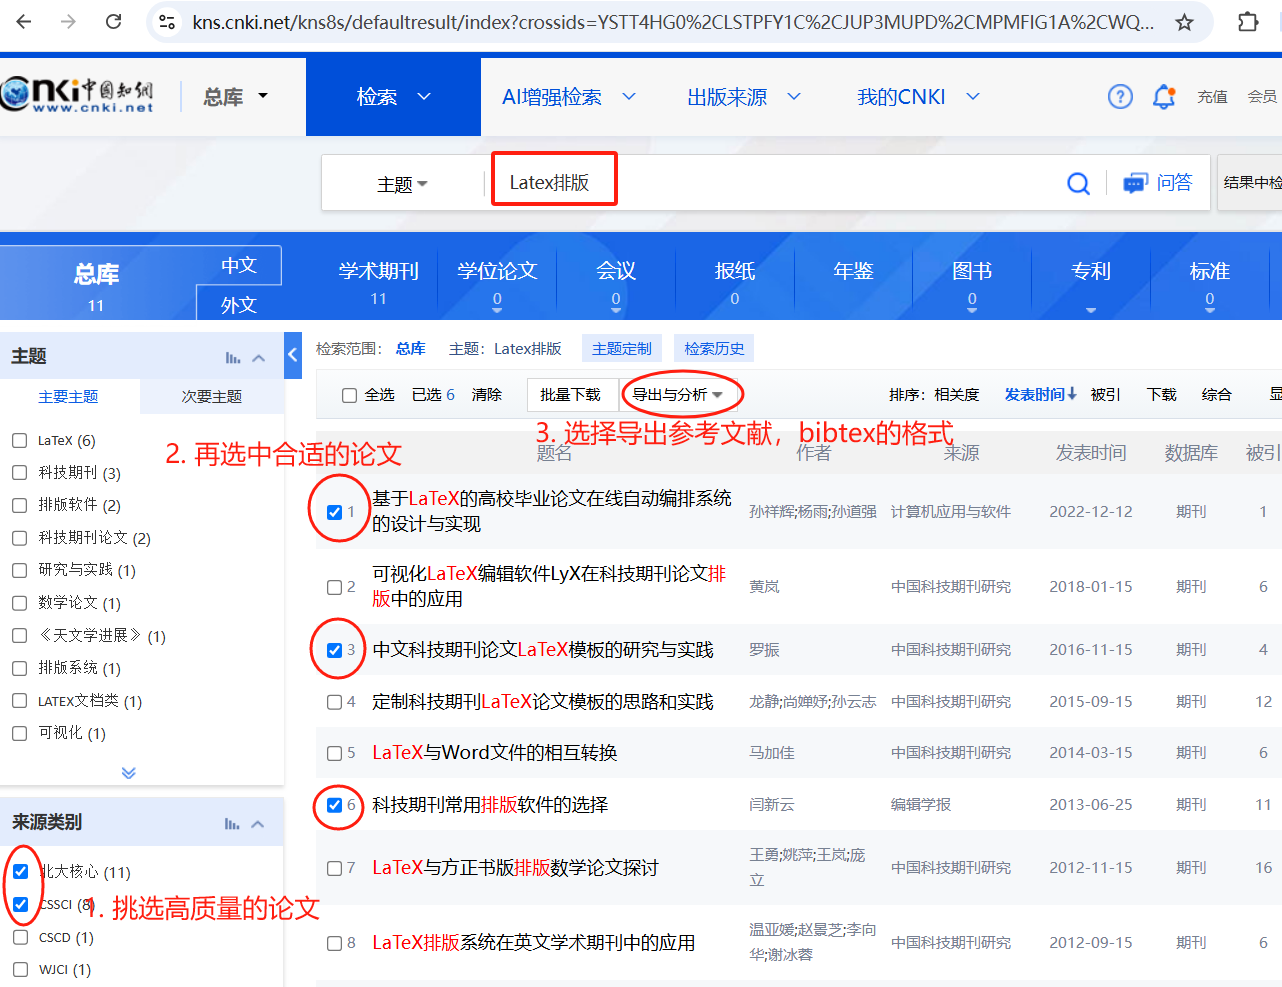
\includegraphics[width=1.0\textwidth]{./图片/论文图片/fig_cnki.png}
	\caption{中国知网查找相应参考文献}\label{fig_cnki}
\end{figure}

所有的参考文献,都要有严格规范的格式,卷期页码等要素齐全,包括标点符号。
文献引用要在文中合适的地方引用,例如,在前人提出的一些方法基础上进行改进时要进行适当引用:早期研究指出,相较于传统文字处理软件,\LaTeX{}在数学符号排版方面具有显著优势\cite{KJYU201010018}。

具体的参考文献要用bibtex的格式保存在另一个文件 reference.bib。
文献最好在中国知网 \href{https://www.cnki.net/}{https://www.cnki.net/} 获取,如图\ref{fig_cnki}。bibtex最好统一去掉每篇论文的doi项。


\section{结论}
本科毕业论文作为本科生培养体系的关键环节,不仅是对学生知识与能力的全面考核,更是培养其科学研究基本功的重要途径。然而,当前学生在毕业论文写作过程中,尤其是在排版方面存在诸多问题,如数学公式排版混乱、图片表格格式欠佳、参考文献管理低效以及代码附录格式不统一等,这些问题严重影响了论文的整体质量。

通过使用本文所介绍的\LaTeX 模板使用方法和排版格式规范,有望帮助学生解决毕业论文排版中的常见问题,提高论文的排版质量和规范性,从而提升学生综合运用专业知识完成毕业论文的能力,为其毕业后的求职立业以及未来撰写专业学术论文奠定良好基础。但需要注意的是,\LaTeX 的使用对于部分学生而言可能存在一定难度,未来可进一步开发更易于上手的辅助工具或提供更详细的教学资源,以促进\LaTeX 在本科毕业论文写作中的更广泛应用。 


	% 需要打开文件“references.bib”来编辑参考文献内容
	\clearpage
	\bibliography{references.bib}
	
	\newpage
	\begin{appendices}
		\renewcommand{\thesection}{附录\Alph{section}}
		\section{第1问的Python求解代码}
		
		\label{append_python}
		
		\begin{lstlisting}[language=Python]
			import numpy as np
			
			# 定义梯度下降函数,用于求解线性回归中的权重参数
			def gradient_descent(X, y, lr=0.01, epochs=100):
			# 获取样本数量 n_samples 和特征数量 n_features
			n_samples, n_features = X.shape
			# 初始化权重向量,将其所有元素初始化为 0
			weights = np.zeros(n_features)
			
			# 开始迭代更新权重,迭代次数为 epochs
			for _ in range(epochs):
			# 计算预测值
			y_pred = X @ weights
			# 计算梯度
			gradient = (2/n_samples) * X.T @ (y_pred - y)
			# 更新权重
			weights -= lr * gradient
			
			# 返回最终学习到的权重向量
			return weights
		\end{lstlisting}
		
	\end{appendices}
\end{document}
